\section{Markerless Recognition}
Several tests were conducted, to assess the performance of the proposed solutions to the tracking and registration problems.\\

\subsection{Colour Search}
The testing phase for the colour scanner began with the RGB colour space. Being the simplest to work with, as the imagery is output in ABGR format (simply RGBA in reverse order), the results were obtained very quickly.\\

\subsubsection{Results}
Searching for colours in the RGB colour space was quite effective, but key factors influenced results negatively.\\

Firstly, lighting affects the reflected colour of an object greatly, and is difficult to account for. In uneven or directed lighting most objects will have gradients across them due to the combination of their shape with the direction of the predominant lighting. This means that when searching for the exact colour of an object, the result gives typically very few pixels on the object matching exactly that colour. Here, by ‘exact colour’ we mean the colour of a selected pixel from the object image. \\

This is the key drawback of the RGB colour space for this type of search, which, theoretically, the HSL colour space could help avoid.\\
Allowing for a range of colours, defined by allowing a specified variance above and below the target colour component values, helps to account for the variation in colour and shade on an object.\\

\subsubsection{Choosing Colours}
Dark colours are poor for tracking. One cause in particular is that dark areas are highly susceptible to noise, which is a key burden of working with low-cost hardware. Dark areas rarely contain the target colour in great quantities, rather a miscellany of colour produced by the sensor. Interestingly, this also causes issues when searching for mid-brightness colours; dark regions occasionally cause flecks of brighter colour which may be in the search range.\\

Brighter colours, therefore, are better for this application. Still, a problem remains in deducing which colour is best for tracking in the target environment. Approaching pragmatically, reds are highly present in photography of people, being a strong component in the colour of skin; and is often a primary indicator of skin in image analysis. Red tones are also prominent in wood, thus appearing regularly in many furnishings. Blue is a prominent colour in NHS equipment, clothing, signage and so forth. Green, however, although ubiquitous in natural scenes, is rarely found in office or medical scenes. Certainly in our testing environment, there were very few green objects.\\

To confirm this, we took a pack of brightly coloured papers and attempted to track them. The pack provided paper in green, yellow, orange and pink. For each colour, we tried using a click-to-match function in our micro-application to see if the paper would be tracked at all, and then assess its visibility at 2.2m distance.\\

\begin{table}
\centering
  \begin{tabular}{| r | r | r | r | r |}
    \hline
    Variance & Green & Orange & Pink & Yellow \\ \hline
    0 & 2 & 4 & 5 & 10\\ \hline
    10 & 1500 & 900 & 1100 & 1300\\ \hline
    20 & \textit{2700} & \textit{2000} & \textit{1900} & \textit{2300}\\ \hline
    30 & \textbf{3300} & 2900 & \textbf{2800} & 2700\\ \hline
    40 & 3900 & 4200 & 9000 & \textbf{3600}\\ \hline
    50 & 4900 & \textbf{7000} & 28000 & 4300\\ \hline
    60 & 7900 & 9800 & 47000 & 5000\\ \hline
  \end{tabular}
    \caption{Filter responses to different colour targets with increasing variance. Italics indicate when the shape was fully and evenly shown. Bold indicates the point at which the target center was most accurately found.}
\end{table}


\subsubsection{HSL Colour Space}
The HSL colour space, by separating hue from shade, potentially allows far greater flexibility under different lighting conditions.
Testing the HSL colour space followed the test mantra laid out by the RGB space experiments. Attempting to track the same sheets of paper, it was found that our mechanism in fact made it harder to track. \\

\begin{table}
\centering
  \begin{tabular}{| r | r | r | r | r |}
    \hline
    Variance & Green & Orange & Pink & Yellow \\ \hline
    0 & 0 & 0 & 0 & 0 \\ \hline
    10 & 100 & 500 & 360 & 150 \\ \hline
    20 & \textit{1200} & 1200 & \textit{2300} & \textit{\textbf{1300}} \\ \hline
    30 & \textbf{1900} & \textit{\textbf{1800}} & 4100 & 2400 \\ \hline
    40 & 3900 & 2200 & 7250 & 3900 \\ \hline
    50 & 4500 & 3100 & 13900 & 5871 \\ \hline
    60 & 5300 & 4600 & 59000 & 7700 \\ \hline
  \end{tabular}
    \caption{Filter responses to different colour targets with increasing variance. Italics indicate when the shape was fully and evenly shown. Bold indicates the point at which the target center was most accurately found.}
\end{table}

The results given by the HSL tracker differ greatly in appearance to those from the RGB tracker. Although a similar mechanism is in place, it appears as though the .HSL tracker is more specific; as the variance is increased, the additional pixels shown are not in contiguous clumps as with the RGB tracker. Rather, the new pixels appear sporadically around the image. This could allow better opportunities for noise removal, as the individual pixels can be cancelled out a lot more easily than blocks.\\

\begin{figure}
\centering
  \begin{tabular}{ c }
    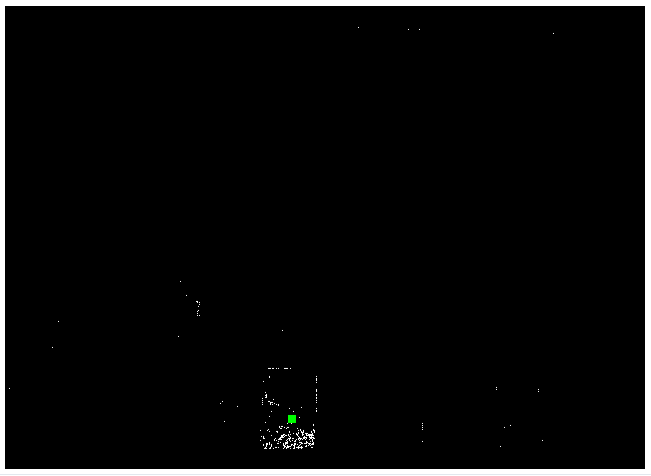
\includegraphics[scale=0.25]{zscreenshots/hsl_green_20}\\ 
    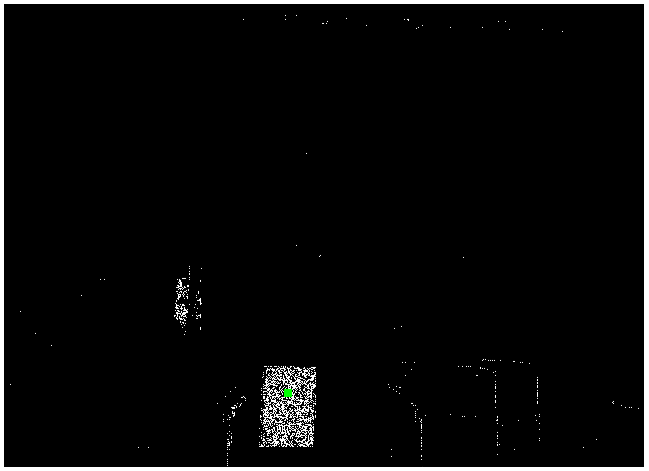
\includegraphics[scale=0.25]{zscreenshots/hsl_green_30}\\ 
    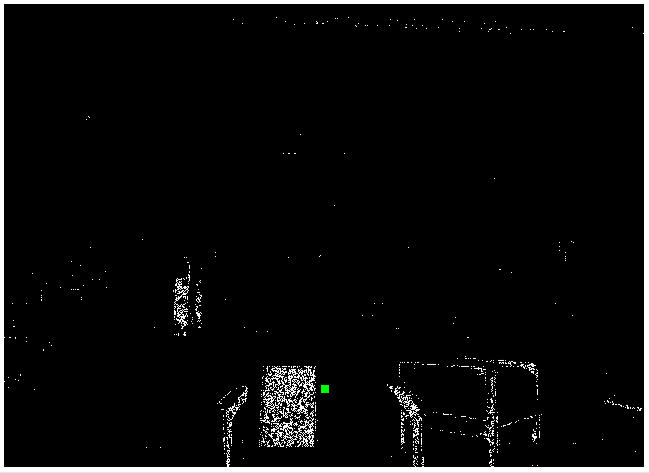
\includegraphics[scale=0.25]{zscreenshots/hsl_green_40}\\ 
    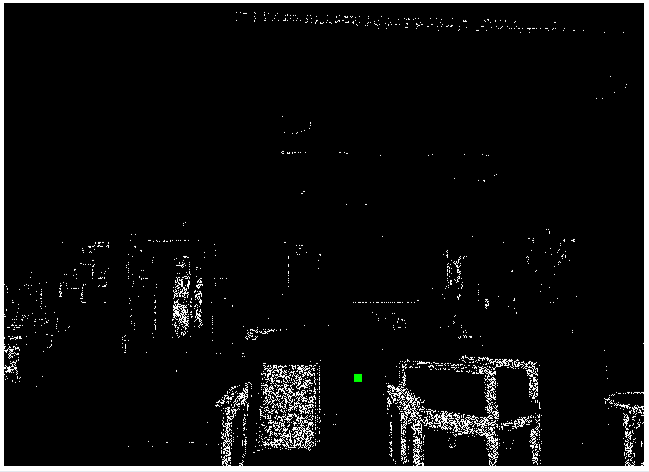
\includegraphics[scale=0.25]{zscreenshots/hsl_green_60}\\ 
    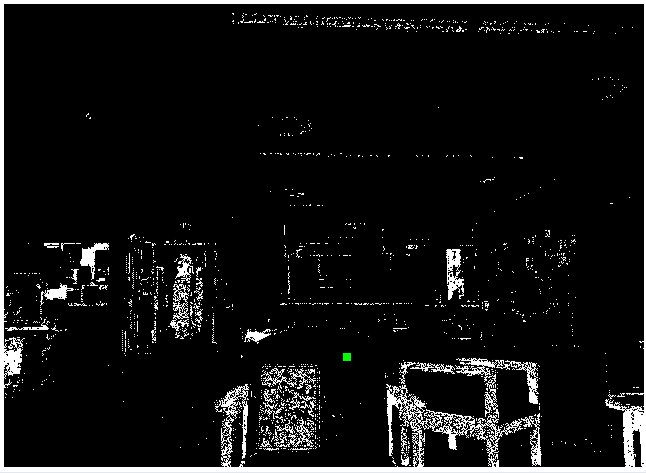
\includegraphics[scale=0.25]{zscreenshots/hsl_green_80}\\
  \end{tabular}
    \caption{Increasing the variance begins to allow colours from the environment.}
\end{figure}

Above 2000 found pixels, the added pixels from variance increase were from the environment more than from the paper. As such, the pink paper never gave a useful result for tracking. A major contributor to this was the slight pinkish hue of the paintwork – never particularly noticed until these tests – which came into range as the increased variance allowed for more subtle colours.\\


\subsubsection{Summary}
Despite key obstacles, tracking in the RGB space worked surprisingly well. Based on a simple, almost primitive, idea, it outperformed the, more complex, HSL colour space search quite competitively. Not only that, but it was much faster to compute. The average frame took 300ms with the RGB search, and 700ms for HSL: a significant difference for a system aiming to provide results in real time.\\

\subsubsection{Lighting}
Lighting, as can be expected, did cause issues. The testing area is subject to strong side lighting from the windows, which causes the angle of the paper to affect perceived colour dramatically. This increased the importance of being able to search for a colour range, rather than a specific colour only.\\

An interesting factor that had an effect on the results was the exposure of the imagery. The exposure time seems to quite drastically affect the colours given – especially for the HSL format imagery, which accounts for lightness and saturation – which reduces the effectiveness of the mechanism. Being beyond our control, it adds a layer of complexity to the HSL imagery which would be very hard to account for.\\

Received light at the sensor is not only affected by the light sources, but the reflecting materials in view. The paper in use, being in texture matte rather than shiny, performed better than some other objects tested, which accentuated the specular lighting. There exist materials with ideal optical properties that would reduce such strong lighting effects further, but this begins to run beyond the scope of the project. Nonetheless, the use of a specific material coating on the sensor could be considered an acceptable modification to allow use of the system, and is worth mention.\\


\subsection{Haar}
The generation of the Haar classifier was to be fraught with complex procedures and intricate setup details. It took several weeks’ research and development to train a classifier at all, before testing could begin.\\

Limitations to this progress were numerous. For classifier use, the PCL library imports a classifier from a file, which is generated externally. To train the classifier, a precise setup must be created, and then generated through use of an executable via an obscure command line process. Further, the training process requires large numbers of training images. The documentation suggested minimal numbers in the order of thousands; a quantity which would take quite some time to collect.\\

The first experiment was, therefore, to find the minimum number of samples required to find a simple object. An application was created to allow the import, classification, and export of images into the correct formats and directory structures required for the training process. A sample of fifty positive, classified images and fifty negative images was found to be sufficient to generate a classifier.\\
Initially, a classifier was generated for a spectacles case – a simple object to hand with a featureful logo and interesting texture. The minimal classifier returned no result.\\
 
This test was important, because it raised important issues. First, would it be feasible to spend many more hours collecting sample data?  Secondly, was a Haar classifier a good choice to use at all? The answer, quickly realised, was no. The restrictions in effectiveness and in training and operation mean that for this application Haar classifiers simply aren’t powerful enough. For clear shapes and structures such as faces, they are well suited. But for this application numerous well-trained classifiers would be required to recognise just one object at various rotations. For the intended real-world application, several different sensors may need to be used and tracked, which raises the issue of training many different classifiers with many input images – too large a problem to be tackled.\\


\subsection{SURF}
The SURF classifier was tested on several different types of imagery to assess its performance. With the placement of synthetic features onto the sensor an allowable possibility, tests were devised to test SURF’s performance on both objects and on synthetic features in order to find a setup with sufficient performance.\\

The test suite included:
\begin{itemize}
\item Detection of objects in photographic imagery
\item Feature detection on synthetic features
\item Detection of synthetic features in synthetic imagery
\item Detection of synthetic features in photographic imagery
\end{itemize}
\\
Detection of objects in photographic imagery
Feature detection on synthetic features
Detection of synthetic features in synthetic imagery
Detection of synthetic features in photographic imagery
\\
\subsubsection{Natural Objects}
Images were taken at 2.2m using a digital camera, with a target object in view. Positive samples were taken of the target object at close range. These images were then run through the SURF classifier.
The testing on objects did not provide the positive results expected. Early testing indicated that, even at close range, what appears by eye to be a featureless object indeed has very few features identified.\\

\begin{figure}
\begin{center}
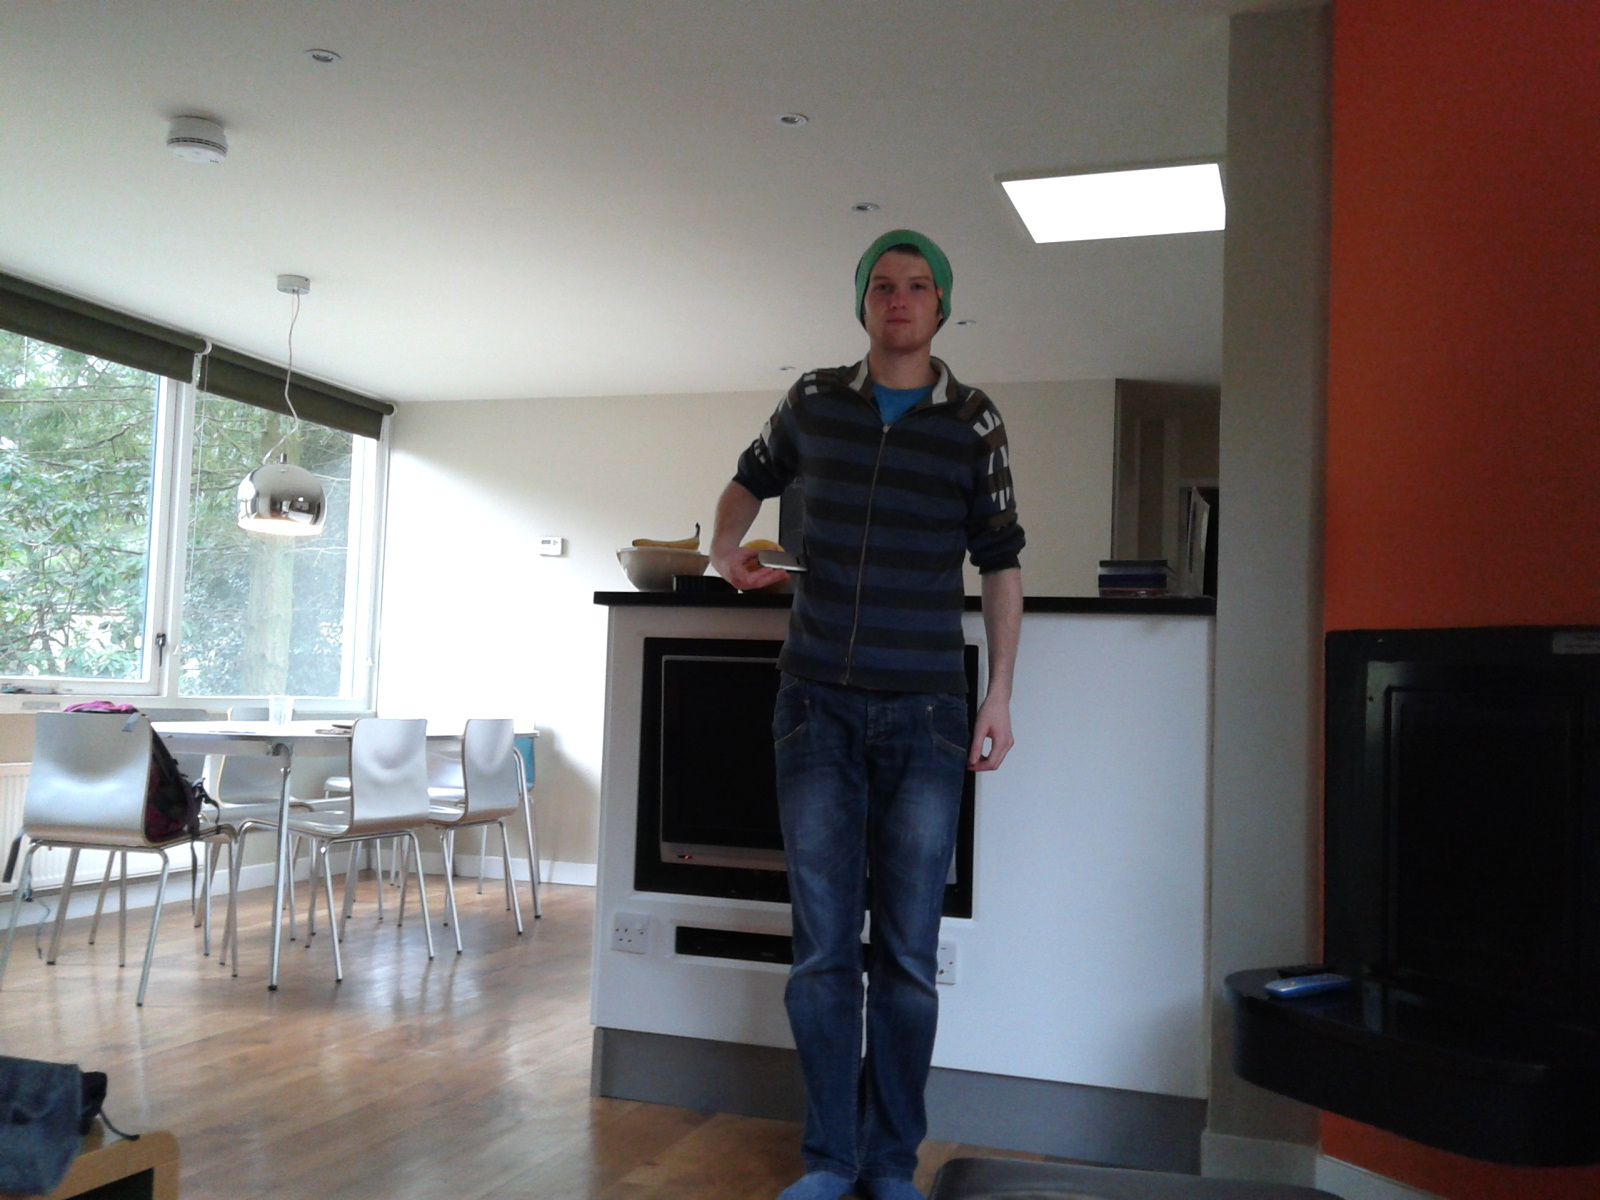
\includegraphics[scale=0.18]{images/20130207_134914.jpg}
\caption{Searching for the target object at distance}
\end{center}
\end{figure}

Part of this is due to SURF’s filtering of features: the initial feature detection will find several thousand features, which are then filtered to retain only those of particular ‘interest’. There is, therefore, no guarantee that the same features will be found in all situations.\\

\begin{figure}
\begin{center}
    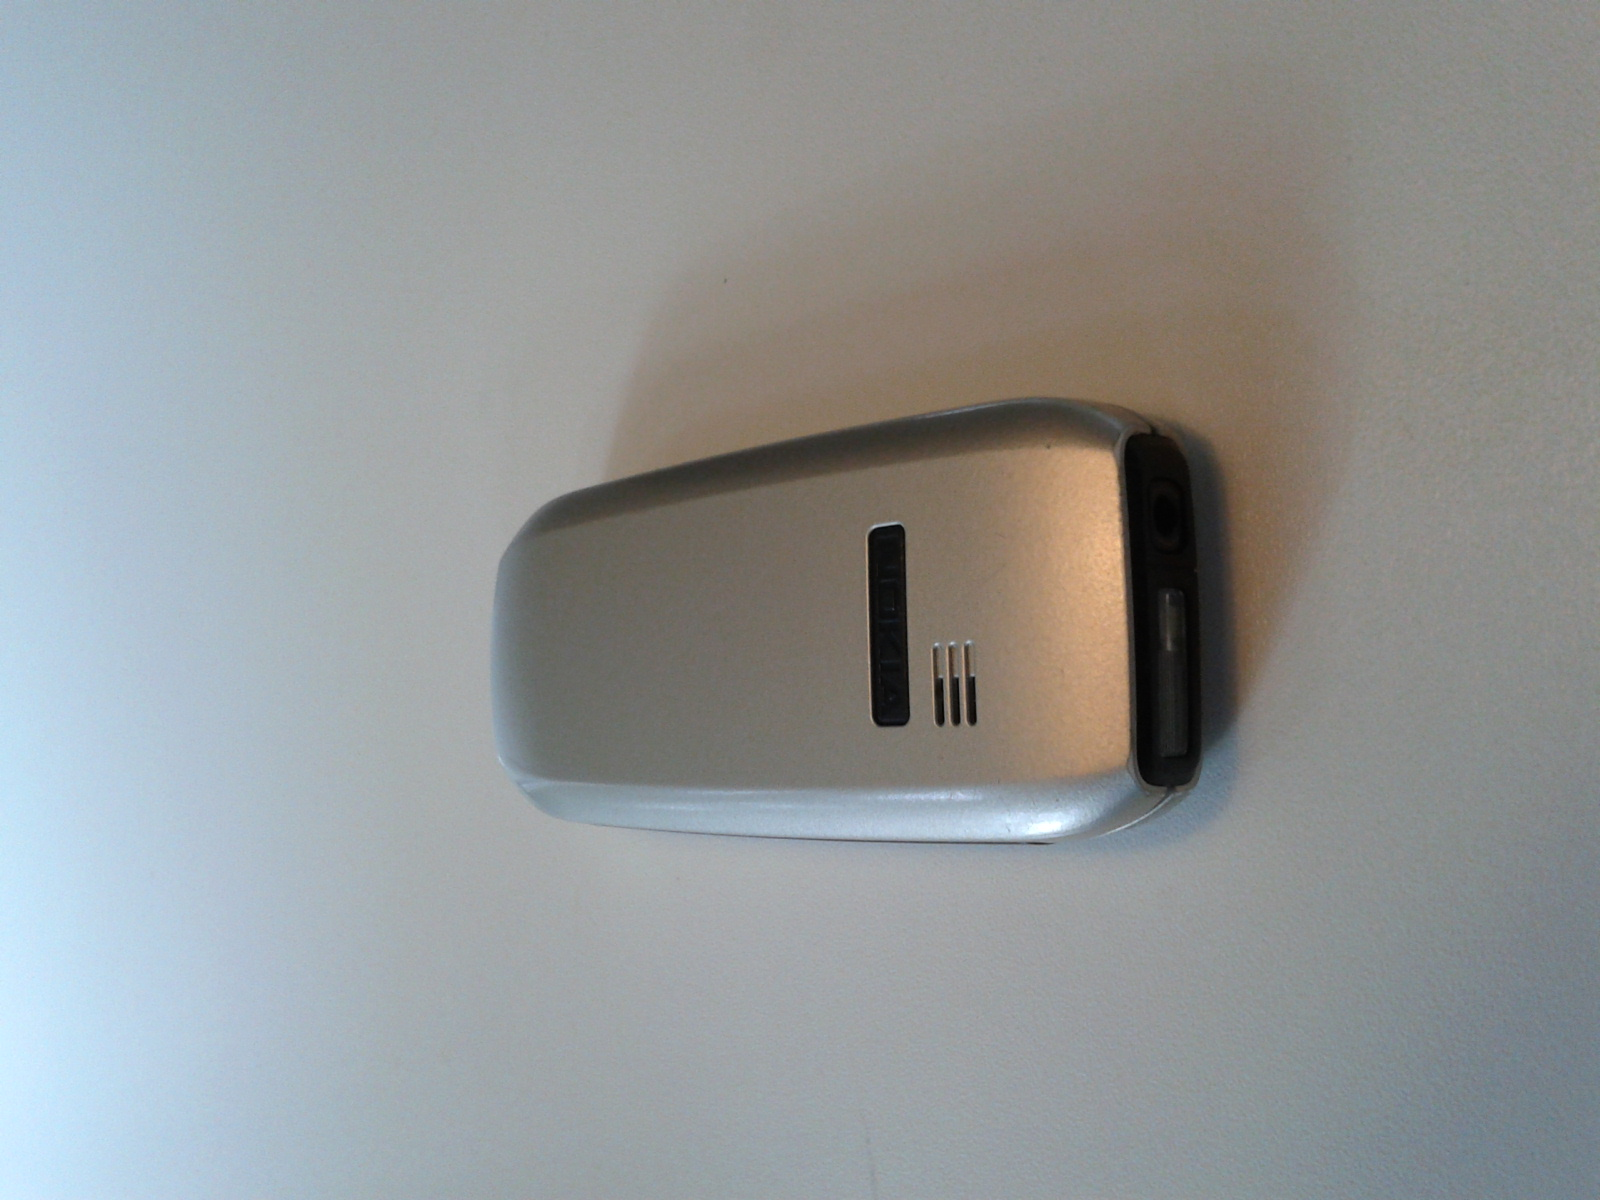
\includegraphics[scale=0.18]{images/20130207_134729.jpg}
    \caption{The target object}
\end{center}
\end{figure}

The target close-ups were cropped and cleaned in order to provide a totally featureless background, such that all features found in the images would be on the target. This is a standard practise. Of further note is the use of target imagery at close range, when the target in the field is at distance. The intention was to see whether this aided feature finding, but clearly it does not. For a high-powered system, it might be possible to have either a series of target images at varying distances, or some internal representation of the target that can be used to model it at any distance, but that is not that case.\\

\subsubsection{Synthetic Features}
Various academic papers and examples show SURF working well, but those examples are typically on carefully constrained example objects, and of course don’t show what SURF didn’t work well on. As it has been shown to work poorly on plain objects, the suggestion to devise some synthetic feature to place upon the target seems sensible. \\

\begin{figure}
\begin{center}
    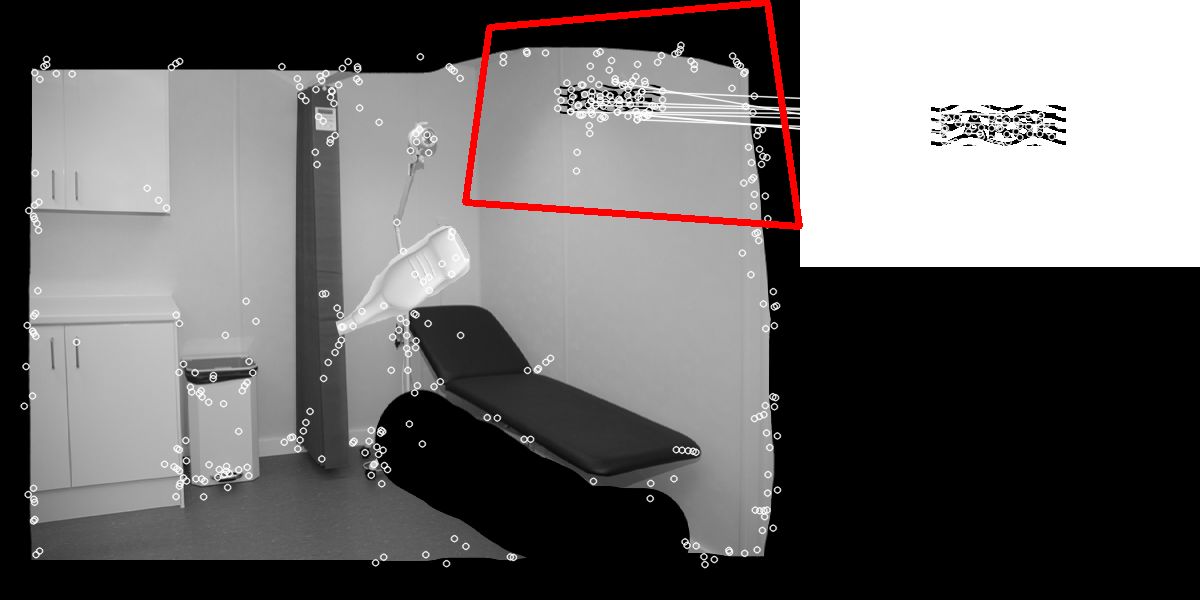
\includegraphics[scale=0.25]{images/synthetic_features_1.png}
    \caption{A synthetic feature inserted into an image, successfully found at near 1:1 scaling.}
\end{center}
\end{figure}

A collection of synthetic features of varying complexity was designed. Each feature was then rescaled in a second image, and the SURF detector used to search for the rescaled feature. The features designed contain different types of features known to be found by the SURF mechanism. \\

The previous problem of unreliable feature sets appeared again at the forefront – when rescaled, the detector found different sets of features. \\

\subsection{The Final Tracking Mechanism}
The system used to track the scanner was the RGB colour search, as it proved under testing to be the most reliable. That said, it was by no means completely reliable. The objects used, particularly under the highly directional lighting of the lab, were subject to specular lighting which reduced the surface area detected. This meant that in around 10\% of frames nothing was found at all. Also with random detected flecks around the room (including edges of plants visible through the glass panel in the door), the feed was quite difficult to work with in its raw form. A very simple mechanism was needed to steady the motion.\\

To perform this the median function was applied on a three frame window. This very effectively covered the holes and anomalies in the data, as neither zeros nor random high or low values would be the median value unless the sensor were detected there for more than one frame - in which case it is possible that the sensor has indeed moved. This made the feed much more stable, but still not completely so.\\

\subsection{Relocating Recorded Scan Positions}
Once stored in the database, recorded scan positions can be re-scanned. The project uses the previously described mechanisms to track the sensor's position relative to the body, except now on every frame. A distance metric is displayed to indicate how close the scanner is to the target position. Again, a capture mechanism is in place to allow the triggering of data capture from a real device.\\

\subsection{Conclusions}
The reliability of the tracking does limit the usability of the system. Overall, what should have been effective display from a set of modern algorithms was hampered by image quality and environmental issues.\\

The low resolution of the imagery, in combination with the environment and the operational properties of the SURF algorithm led to its poor result. As for the Haar classifier, it was quite possibly never going to work. It is difficult to assess how algorithms will perform, without a very full understanding of their operation. Such also are the difficulties of understanding how an algorithm will perform in different applications, scenarios and datasets, that often the best, and only, way to find out is to try.\\

Having made great effort to see a robust, feature-driven algorithm solve the problem, it is disappointing to find that our selections were ineffective, and that it is the almost trivial colour search in the RGB format that provided the only usable solution.\\

\subsection{Further development}
The RGB colour search was rightly the method chosen to drive the sensor tracking. Although lighting affects it so much, it is a fairly stable mechanism under consistent lighting, and is very easy to reconfigure if necessary; much unlike the ordeal required to train a new Haar classifier.\\

\subsubsection{Improving the tracking}
Part of the problem with the RGB tracking mechanism was that the whole environment was searched. One improvement, which was attempted as an aside but not completed, would be to use the depth data as a mask. Removing from the colour frame all regions behind the subjects would reduce drastically the noise present in the image, making tracking simpler whilst also more accurate.\\

The ability to control the lighting itself would be a highly desirable addition.\\

